\documentclass{beamer}
 
\usepackage[utf8]{inputenc}
\usepackage{graphicx}
\usepackage{tabularx}
\usepackage{amssymb}
\usepackage{verbatim}
\usepackage{fancyvrb}
\usepackage{amsmath}
\usepackage{bm}
\usepackage{tikz}
\usetheme{Madrid}
\newcommand{\Perp}{\perp \! \! \! \perp}


\title[BST 234]{BST 234: Lab - 3}
\author[Divy Kangeyan]{Divy Kangeyan}
%\institute{Stat 365R}
\date{\today}

\begin{document}
	%
	
	\begin{frame}
		\titlepage
	\end{frame}
	
	%IF YOU INCLUDE TABLE OF CONTENTS
	%\section[Outline]{}
	%\frame{\tableofcontents}
	
\section{Python}

\begin{frame}
\frametitle{Classes in Python}

\begin{itemize}
\item Classes define objects and their associated methods
\item class object is defined as \texttt{class <name>:}

\end{itemize}




\end{frame}



\begin{frame}
\frametitle{Class Objects}

\begin{itemize}
\item Class objects support two operations
\begin{enumerate}
\item Attribute references
\item Instantiation
\end{enumerate}

\item We need to create an instance of the class and then we may reference its various attributes

\end{itemize}
\end{frame}


\begin{frame}
\frametitle{Class Objects}

 
\begin{itemize}
\item Class
\pause
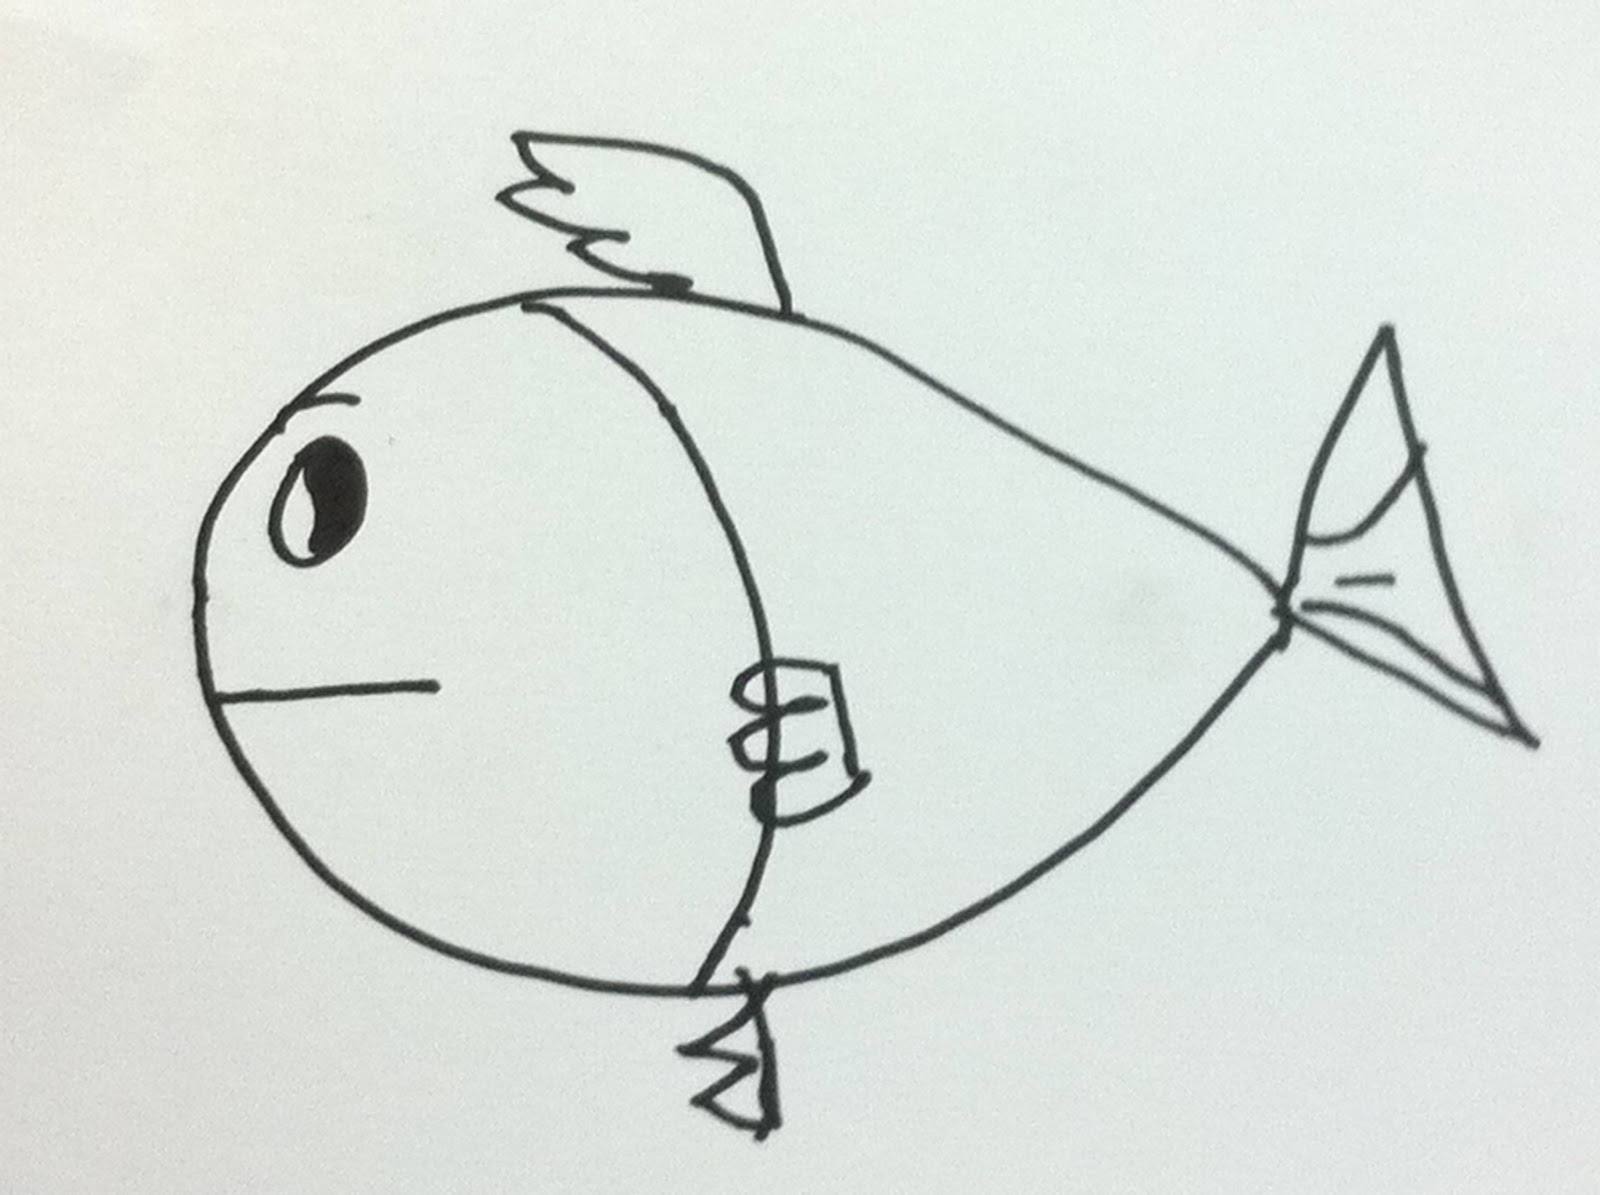
\includegraphics[width=1.2in]{fish.jpg}
\pause
\item Class objects support two operations
\pause
\begin{enumerate}
\item Attribute references :  \pause \texttt{has gills, has scales}
\item Instantiation:  \pause 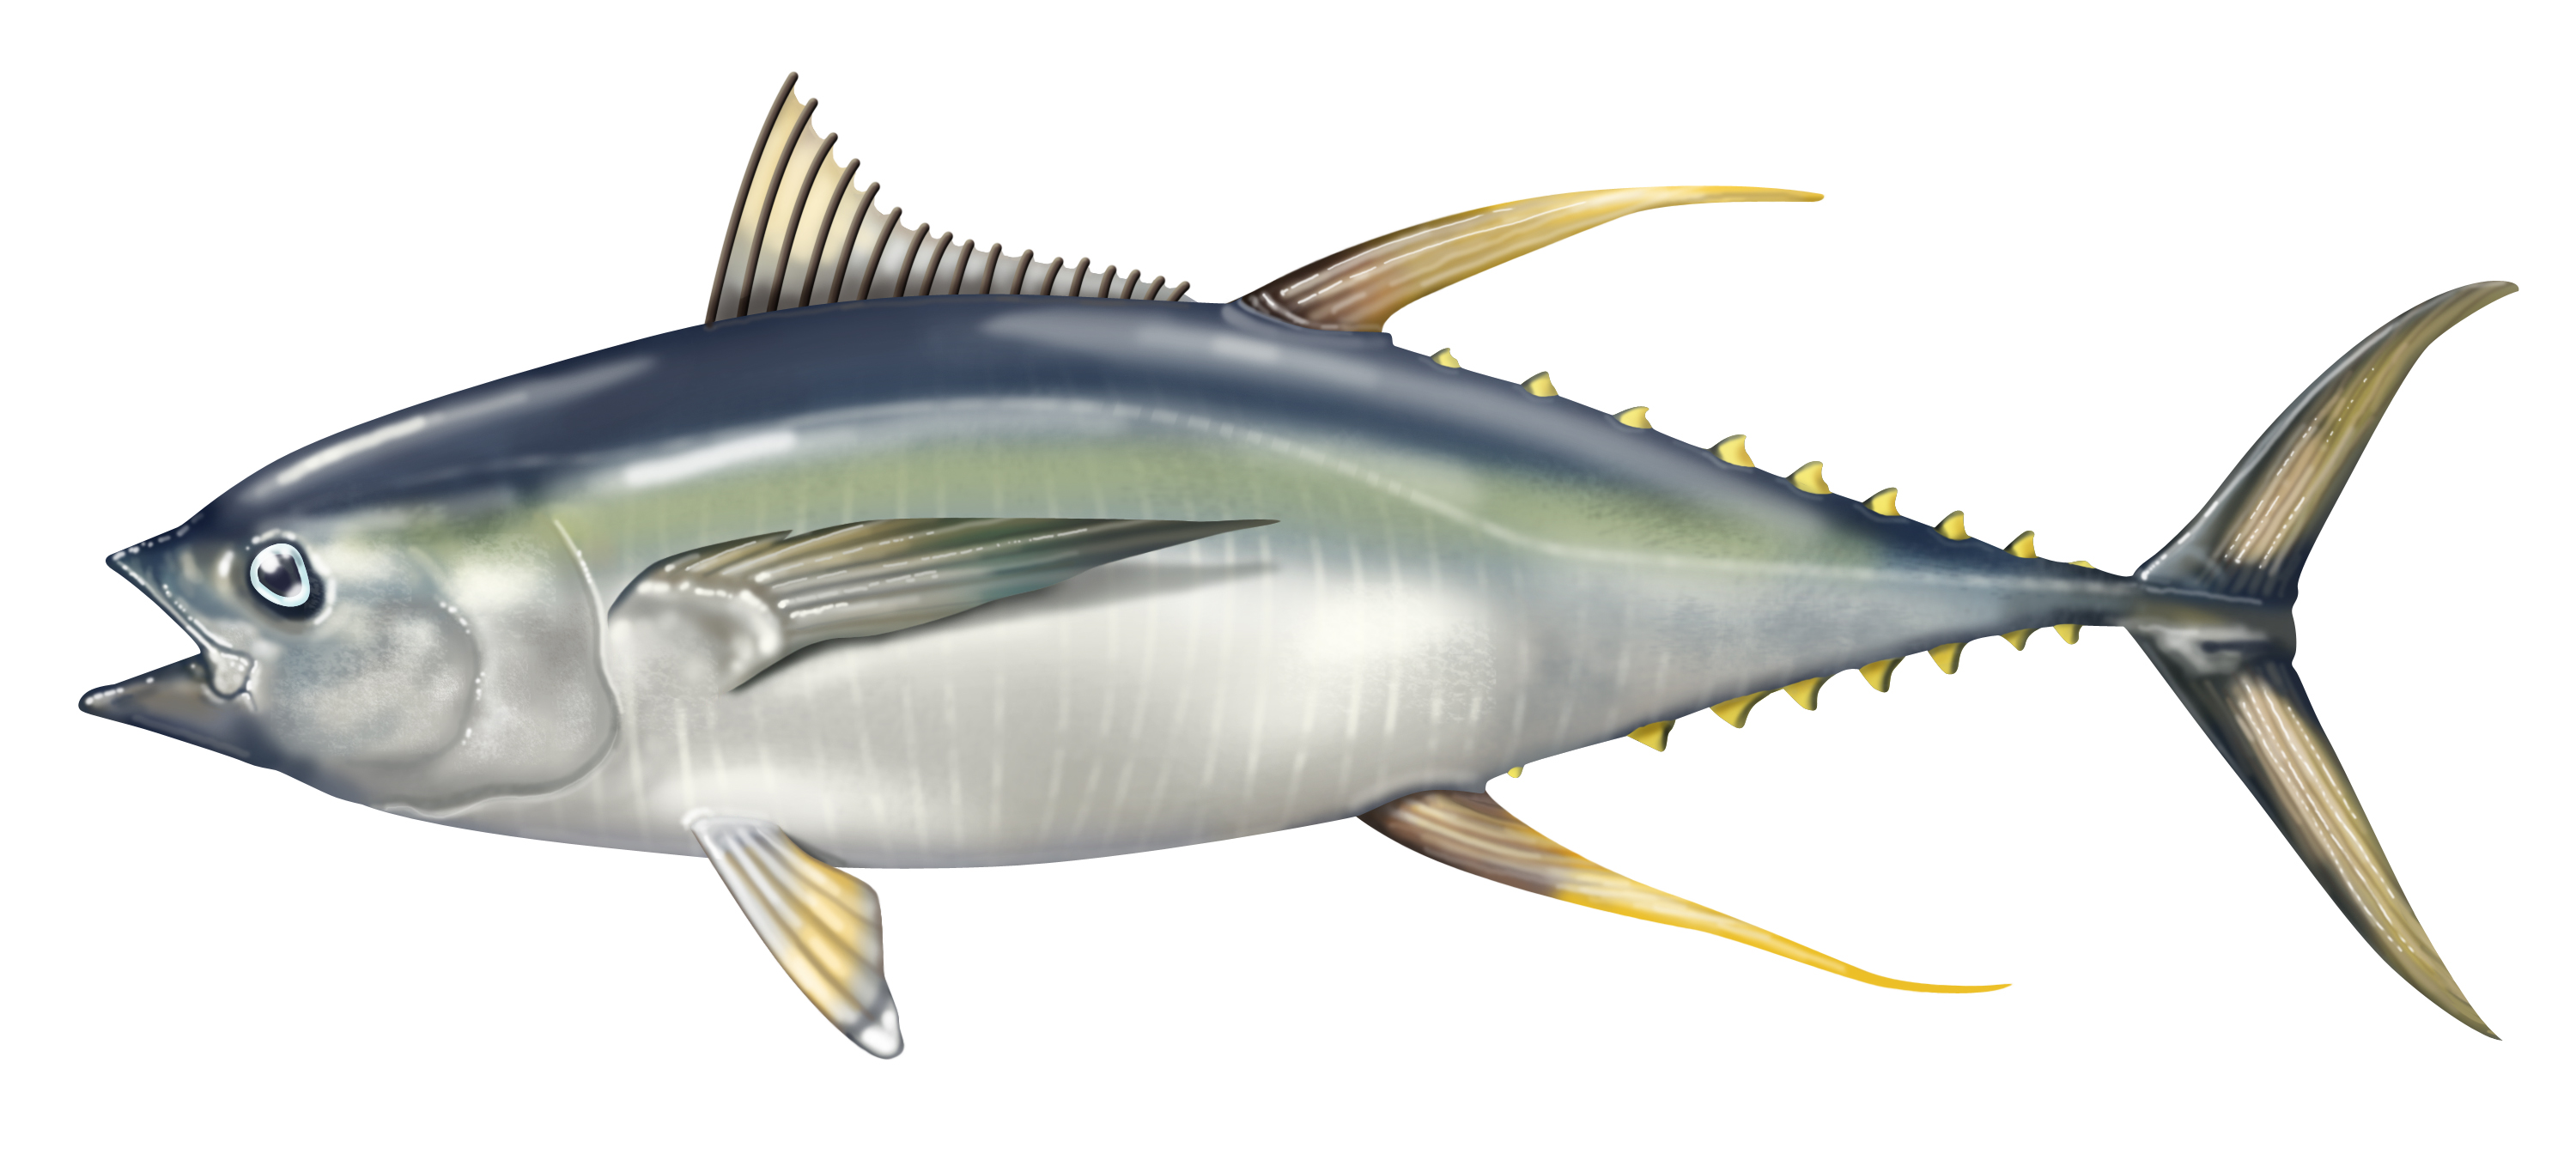
\includegraphics[width=1.2in]{tuna.jpg}
\end{enumerate}

\end{itemize}




\end{frame}


\begin{frame}
\frametitle{Class Instantiation}

\begin{itemize}


\item We need to create an instance of the class and then we may reference its various attributes

\end{itemize}


\end{frame}



\begin{frame}[fragile]
\frametitle{Class Instantiation}



\begin{Verbatim}
class MaxHeap(object):
	#construct - empty array
	def __init__(self, data = []):
		self.data = data
\end{Verbatim}

Calling the class

\begin{Verbatim}
x = MaxHeap()
data = x.data
\end{Verbatim}
\end{frame}


\begin{frame}
\frametitle{Attribute Reference}

\begin{itemize}
\item Given an instance, we may reference attributes (assign, retrieve, delete)
\item Two types of attributes:
\begin{enumerate}
\item Data attributes
\item Methods
\end{enumerate}

\end{itemize}


\end{frame}



\begin{frame}[fragile]
\frametitle{Attribute reference}



\begin{Verbatim}
class MaxHeap(object):
	#construct - empty array
	def __init__(self, data = []):
		self.data=data
	
	def isEmpty(self):
		return(len(self.data) == 0)
		
\end{Verbatim}


\end{frame}



\begin{frame}
\frametitle{Class Vs. Instance variables}

\begin{itemize}
\item We saw how to reference methods on the previous slides
\item Two types of variables exist
\pause
\begin{enumerate}
\item Class variable(e.g. has gills, has scales) \pause
\item Instance variable(e.g. color of a muscle tissue ranges from pink to dark red, streamlined body)
\end{enumerate}
\pause
\item Class variables are shared by all instances of the class
\item Instance variable are unique to each call
\end{itemize}




\end{frame}

\begin{frame}[fragile]
\frametitle{Class Vs. Instance variables}

\begin{Verbatim}
class Fish:
  self.gills = True
  self.scales = True
  def __init__(self, muscle_color, body_type):
    self.muscle_color = muscle_color
    self.body_type = body_type

		
\end{Verbatim}




\end{frame}


\begin{frame}
\frametitle{Summary}

\begin{itemize}
\item Classes provide a structure for a process with associated methods and objects
\item Attribute references and instantiation are operations supported by a class object
\item Data attributes and methods are two types of attributes
\item There are two types of variables: class variable (shared by all instance of a class) and instance variable (unique to each instantiation)
\end{itemize}


\end{frame}



\end{document}